% Progress report and retrieval plan -- compile with pdfLaTeX (Overleaf default).
% Self-contained: no external files, no BibTeX.
\documentclass[11pt,a4paper]{article}

\usepackage[T1]{fontenc}
\usepackage[utf8]{inputenc}
\usepackage{lmodern}
\usepackage[margin=2.25cm]{geometry}
\usepackage{microtype}
\usepackage{amsmath}
\usepackage{booktabs}
\usepackage{tabularx}
\usepackage{enumitem}
\usepackage{xcolor}
\usepackage{tikz}
\usetikzlibrary{arrows.meta,positioning,fit,calc}
\usepackage{caption}
\usepackage[hidelinks]{hyperref}

\usepackage{titlesec}
\titlespacing*{\section}{0pt}{1.2ex plus .3ex}{0.6ex plus .2ex}
\titlespacing*{\subsection}{0pt}{0.9ex plus .2ex}{0.4ex plus .1ex}
\titleformat{\section}{\large\bfseries}{\thesection}{0.6em}{}
\titleformat{\subsection}{\normalsize\bfseries}{\thesubsection}{0.5em}{}
\setlength{\parskip}{2pt}
\setlength{\emergencystretch}{2.2em}
\setlist[itemize]{itemsep=1pt,topsep=2pt,parsep=0pt,leftmargin=1.15em}
\setlist[enumerate]{itemsep=1pt,topsep=2pt,parsep=0pt,leftmargin=1.4em}
\captionsetup{font=small,labelfont=bf,skip=4pt}
\newcommand{\code}[1]{\texttt{#1}}

% One colour carries one meaning throughout: blue = part of the retrieval path (present only when RAG is on).
\definecolor{ragblue}{RGB}{31,94,170}
\colorlet{ragfill}{ragblue!7}
\colorlet{edge}{black!55}
\tikzset{
  box/.style={draw=edge, rounded corners=2pt, align=center, inner sep=3pt,
              minimum height=1.05cm, fill=black!3, font=\scriptsize},
  ragbox/.style={box, draw=ragblue, fill=ragfill, line width=0.7pt},
  arr/.style={-{Latex[length=1.8mm]}, draw=black!65, semithick},
  lbl/.style={font=\scriptsize, fill=white, inner sep=1pt},
}

\title{\vspace{-1.2em}\textbf{An LLM Agent for Competitive Pok\'emon:}\\[0.1em]
\textbf{Progress Report and Retrieval Plan}\\[0.35em]
\large From a minimal prompting demo to a retrieval-augmented battle agent}
\author{CISC7404 \emph{AI-Trustworthy} Project Team\\University of Macau}
\date{3 November 2026 (revised 7 November 2026)}

\begin{document}
\maketitle
\vspace{-2.2em}

\begin{abstract}
\noindent
We report on the first three weeks of a course project that builds a large language model (LLM) agent for
competitive Pok\'emon (\code{gen9ou}) on Pok\'emon Showdown, and we fix the plan for its central question:
does retrieval-augmented generation (RAG) improve the agent's decisions? The agent has evolved from a
one-call-per-turn demo into a tool-using agent built on \code{pi-python-core}, with OpenCode Go as the
default model adapter and a deterministic move/ability/item/rule card corpus. For the remaining work we
separate domain knowledge from the battle prompt. Knowledge about moves, abilities, items, battle rules and
common opponent sets moves into a knowledge base of 3{,}030 entity cards, indexed by \code{pi-knowledge}
and exposed to the model through a single retrieval tool. The default local embedding model is
\code{e5-small}; Qwen3-Embedding-0.6B is an optional OpenAI-compatible endpoint. The evaluation compares
the same agent with and without that tool and measures three things in turn: whether retrieval returns the
right card, whether the model uses it, and whether its decisions improve.
\end{abstract}

\section{Introduction}

At every turn of a Pok\'emon battle the agent observes the state, chooses one legal action (a move, a switch,
or a Terastallized move) and repeats until one side has no Pok\'emon left. Beyond winning, the agent must be
\emph{trustworthy} in a sense that can be checked from its own logs. Four commitments shape the code base:

\begin{itemize}
  \item \textbf{Information legality.} The agent sees only what a human player sees: team preview, revealed
        opponent information and the public battle history.
  \item \textbf{Grounded arithmetic.} Damage, speed order and knock-out chances come from the battle
        simulator, not from the model's own reasoning.
  \item \textbf{Reproducible decisions.} Every turn is logged with its prompt size, tool calls, answer,
        reasoning and token usage, so a lost game can be replayed from the trace.
  \item \textbf{Fail-safe control.} A failed parse, tool or API call degrades to a legal move; it never ends
        the battle.
\end{itemize}

\noindent
The project now addresses one research question:

\begin{quote}
\emph{Given an agent that already receives the battle state and simulator-computed quantities, does
on-demand retrieval of domain knowledge improve its decisions, and at what cost in latency and tokens?}
\end{quote}

\noindent
Section~\ref{sec:arch} describes the system, Sections~\ref{sec:progress} and~\ref{sec:traces} summarise
progress and what the decision traces show, Section~\ref{sec:rag} presents the retrieval-augmented design~\cite{rag},
Section~\ref{sec:eval} the evaluation, and Section~\ref{sec:schedule} the schedule.

\section{System architecture}
\label{sec:arch}

The system has four layers: a \emph{battle server}, a \emph{client player} built on \code{poke-env}~\cite{pokeenv}, a
\emph{decision layer} that runs one LLM agent per turn with tools, and an \emph{observation layer} that writes
the decision trace. Figure~\ref{fig:arch} shows the data flow in its planned form; the components drawn in
blue are the retrieval path, which is the only difference between the two experimental arms.

\begin{figure}[t]
\centering
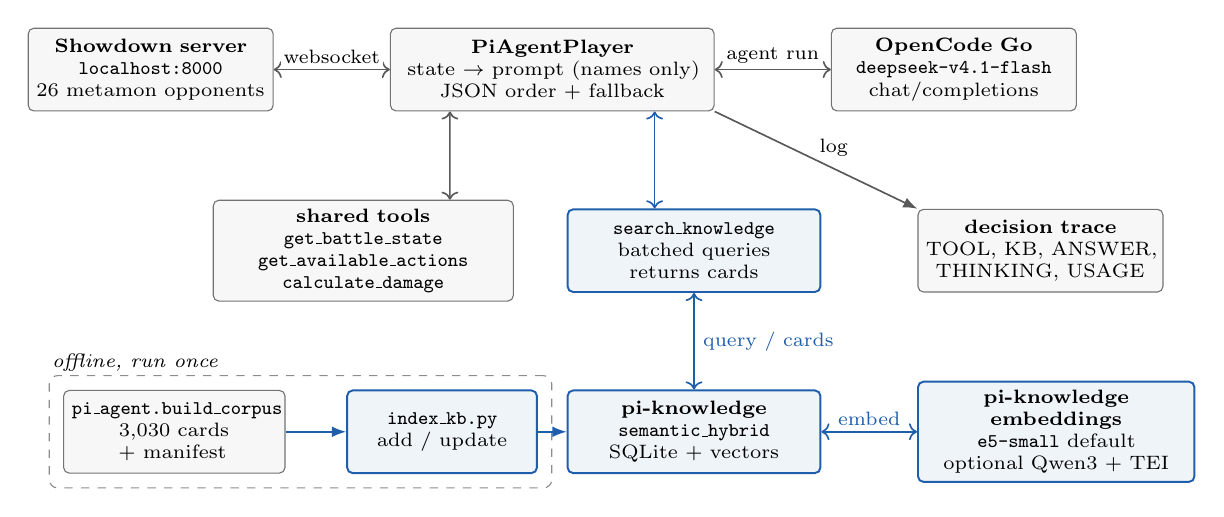
\begin{tikzpicture}[x=1cm, y=1cm]
  % decision loop (top row)
  \node[box, text width=2.9cm] (srv)   at (1.2,0)  {\textbf{Showdown server}\\ \code{localhost:8000}\\ 26 metamon opponents};
  \node[box, text width=3.9cm] (agent) at (6.3,0)  {\textbf{PiAgentPlayer}\\ state $\rightarrow$ prompt (names only)\\ JSON order + fallback};
  \node[box, text width=2.9cm] (llm)   at (11.4,0) {\textbf{OpenCode Go}\\ \code{deepseek-v4.1-flash}\\ chat/completions};
  % tools and trace (middle row)
  \node[box, text width=3.6cm] (tools) at (3.9,-2.3) {\textbf{shared tools}\\ \code{get\_battle\_state}\\ \code{get\_available\_actions}\\ \code{calculate\_damage}};
  \node[ragbox, text width=3.0cm] (rag) at (8.1,-2.3) {\textbf{\code{search\_knowledge}}\\ batched queries\\ returns cards};
  \node[box, text width=2.9cm] (log)   at (12.5,-2.3) {\textbf{decision trace}\\ TOOL, KB, ANSWER,\\ THINKING, USAGE};
  % retrieval stack and offline indexing (bottom row)
  \node[ragbox, text width=3.0cm] (pk)  at (8.1,-4.6)  {\textbf{pi-knowledge}\\ \code{semantic\_hybrid}\\ SQLite + vectors};
  \node[ragbox, text width=3.3cm] (tei) at (12.7,-4.6) {\textbf{pi-knowledge embeddings}\\ \code{e5-small} default\\ optional Qwen3 + TEI};
  \node[box, text width=2.6cm] (cards) at (1.5,-4.6) {\textbf{\code{pi\_agent.build\_corpus}}\\ 3{,}030 cards\\ + manifest};
  \node[ragbox, text width=2.2cm] (index) at (4.9,-4.6) {\textbf{\code{index\_kb.py}}\\ add / update};
  \node[draw=black!45, dashed, rounded corners=3pt, inner sep=5pt, fit=(cards)(index),
        label={[font=\scriptsize\itshape, anchor=south west, inner sep=1pt]north west:offline, run once}] {};

  \draw[arr, <->] (srv) -- node[lbl, above=1pt] {websocket} (agent);
  \draw[arr, <->] (agent) -- node[lbl, above=1pt] {agent run} (llm);
  \draw[arr, <->] ([xshift=-1.3cm]agent.south) -- ([xshift=1.1cm]tools.north);
  \draw[arr, <->, ragblue] ([xshift=1.3cm]agent.south) -- ([xshift=-0.5cm]rag.north);
  \draw[arr] (agent.south east) -- node[lbl, above right=0pt] {log} (log.north west);
  \draw[arr, <->, ragblue] (rag) -- node[lbl, right=2pt] {query / cards} (pk);
  \draw[arr, <->, ragblue] (pk) -- node[lbl, above=1pt] {embed} (tei);
  \draw[arr, ragblue] (cards) -- (index);
  \draw[arr, ragblue] (index) -- (pk);
\end{tikzpicture}
\caption{One battle turn in the planned system. Blue components form the retrieval path and exist only in
the \code{rag=on} arm; everything else is identical in both arms. The dashed group runs once, before any game.}
\label{fig:arch}
\end{figure}

\subsection{Server and opponent pool}
The public PokeAgent Challenge server~\cite{challenge} is permanently closed, so games run on a local Pok\'emon Showdown server
(\code{localhost:8000}, format \code{gen9ou}). The opponent pool, maintained in a companion repository, keeps
26 metamon players online: 10 reinforcement-learning policies and 16 heuristic or imitation-learning baselines.
Damage uses metamon's battle simulator and its damage engine, not a second simulator.

\subsection{Turn loop and tools}
\code{pi\_agent.player.create\_player} wraps a poke-env Player. The Pi agent sees one reduced state message,
a list of legal actions, and tools shared across turns. It maps the chosen action to a Showdown order with
\code{player.create\_order}; a non-JSON answer gets a repair prompt, and a still-illegal answer falls back to
the highest-power legal move. Model and tool budgets come from environment variables, defaults
\code{max\_model\_requests=8} and \code{max\_tool\_calls=8} with a 240\,s run timeout.
Every tool returns readable text and catches its own exceptions, so a failed tool is data for the model
rather than a crash.

\subsection{Local ranks and checks}
The \code{pi\_agent} runtime in this checkout can run the pool end to end:
\begin{itemize}
  \item \code{python -m pi\_agent.build\_corpus} produces deterministic cards and a SHA-256 manifest.
  \item \code{python -m pi\_agent.index\_kb} builds or refreshes the local \code{pi-knowledge} index.
  \item \code{python -m pi\_agent.knowledge\_doctor} reports retrieval health.
  \item \code{python -m pi\_agent.check} runs offline checks without Showdown, the OpenCode API, or an
        embedding server.
\end{itemize}
\code{python -m pi\_agent.run --opponent MM-Kakuna --rag on|off} exercises both arms against one pool player.

\subsection{Model backend and traces}
\code{player\_pool.llm\_client} is the OpenCode-compatible model client used in this checkout. It keeps one
persistent session per game, sends the OpenCode-required \code{x-opencode-session} and a real
\code{User-Agent}, and exposes \code{usage.opencode.cost/billing\_source/allowance} so the trace can log
spend. For pay-as-you-go, use \code{provider="opencode"} and
\code{base\_url=https://opencode.ai/inference}.

Each agent run appends one block to the trace: a header (turn, model, thinking level, prompt size, tools),
one line per tool call, the final answer, the reasoning, and aggregated usage and latency. The retrieval
design adds the experimental arm and the knowledge-base signature to the header, and one \code{KB} line per
retrieval call (queries, returned cards, scores, misses and latency).

\section{Progress to date}
\label{sec:progress}

The agent has gone through three generations. The first is a demo with one chat call per
turn and a hand-written prompt; it asks the model to do arithmetic in its head. The second ports the
Pok\'eChamp harness~\cite{pokechamp} to an OpenCode-style Chat Completions endpoint and brings a structured
state prompt, an approximate damage calculator and a trace format, but in its default \code{io} mode it
cannot yet call tools. The third generation is the current code base, \code{pi\_agent/}: it is a
\code{pi-python-core}~\cite{pi} player with high-level tools (state, actions, damage, knowledge), an OpenCode
Go model backend, and a deterministic \code{pi-knowledge}-based RAG stack. Table~\ref{tab:gens} summarises
them; it uses the turn counts from an earlier harness register only where present.

\begin{table}[t]
\centering
\small
\caption{Generations of the agent. ``Decisions'' counts logged turns, not games; new code has no trace yet.}
\label{tab:gens}
\begin{tabularx}{\textwidth}{@{}>{\raggedright\arraybackslash}p{2.1cm} >{\raggedright\arraybackslash}X >{\raggedleft\arraybackslash}p{1.6cm}@{}}
\toprule
\textbf{Generation} & \textbf{What it adds} & \textbf{Decisions} \\
\midrule
v0 demo    & One chat call per turn, hand-written prompt with type and speed hints, integer action index
             & 128 \\
v1 harness & Structured state prompt, approximate \code{LocalSim} damage, RAG wire format, 8192-token
             thinking budget, retry on truncation & 61 \\
v2 agent   & \code{pi-python-core} player with callable tools, named JSON contract, repair and fallback,
             local \code{gen9ou} pool, \code{pi-knowledge} bridge, generated knowledge card set
             & --- \\
\bottomrule
\end{tabularx}
\end{table}

Engineering milestones: non-AI baseline on 13 October; first public-server games with thinking enabled on
16 October; harness port on 18 October; \code{pi\_agent} and the knowledge bridge on 23 October;
\code{pi\_agent} tool-plus-knowledge integration, deterministic card generation and offline checks on
7 November.

\section{What the decision traces show}
\label{sec:traces}

\textbf{Parsing is not the bottleneck.} The demo produced 128 valid decisions in a row, and the current agent
adds a tolerant extractor, a repair prompt and a deterministic fallback.

\textbf{Reasoning dominates cost.} Across 60 harness decisions the mean prompt was about 2.1k tokens and the
mean completion about 3.0k. Six responses hit the output cap and were retried with a doubled budget. Latency
averaged 18.7\,s per call (maximum 73.2\,s), within the 150\,s turn limit but slow enough that long runs belong
off-peak.

\textbf{Battle length varies widely.} Five logged games contained 2, 2, 12, 7 and 38 decisions, so per-turn
statistics must be averaged per battle before they are pooled.

\textbf{Arithmetic, not planning, causes stalls.} The recurring failure is a sound plan abandoned after the
model re-derives a damage roll and doubts it; \code{calculate\_damage} exists to break this loop.

These observations concern efficiency. They are handled by tuning that is fixed before the comparison
(Section~\ref{sec:tuning}), not by the comparison itself.

\section{Retrieval-augmented design}
\label{sec:rag}

\subsection{What stays in the prompt}
The current prompt mixes three kinds of content (Table~\ref{tab:split}). Only domain knowledge is static and
needed on some turns but not others, which is what retrieval is for. Simulator quantities stay in the prompt
and in \code{calculate\_damage}: retrieving them could fail and would turn exact arithmetic back into guessing.
Both arms therefore use the same reduced prompt, which keeps entity names (the keys the model searches with)
but drops their descriptions. \code{get\_battle\_state} returns the same reduced text; otherwise the
\code{rag=off} arm could recover the removed knowledge through that tool.

\begin{table}[t]
\centering
\small
\caption{Where each kind of prompt content lives after the change.}
\label{tab:split}
\begin{tabularx}{\textwidth}{@{}>{\raggedright\arraybackslash}p{3.0cm} >{\raggedright\arraybackslash}X >{\raggedright\arraybackslash}p{3.6cm}@{}}
\toprule
\textbf{Content} & \textbf{Examples} & \textbf{Location} \\
\midrule
Battle state          & history, HP, status, boosts, hazards, legal actions & prompt (both arms) \\
Simulator quantities  & stats, effective power, type multipliers, speed order, KO turns & prompt and \code{calculate\_damage} \\
\textcolor{ragblue}{Domain knowledge} & move, ability and item effects; rules; likely opponent sets
                      & \textcolor{ragblue}{knowledge base} (\code{rag=on} only) \\
\bottomrule
\end{tabularx}
\end{table}

\subsection{Knowledge base}
Each entity becomes one Markdown card, and each card is one retrieval unit of at most about 1{,}000
characters (Table~\ref{tab:kb}). Cards are generated deterministically by \code{pi\_agent.build\_corpus}
from the Showdown Pok\'edex, Showdown text data, and metamon's \code{gen9ou} static tables. A card's title
holds both the identifier and the display name (\code{greattusk} and \emph{Great Tusk}), and its file path
encodes the category, so a search can be restricted to one category. Currently there are no usage-stats
entries; species cards hold public Pok\'edex data and the Showdown text data supplies move and ability
effects. The generator writes a manifest of source files and SHA-256 hashes.

\begin{table}[t]
\centering
\small
\caption{Composition of the generated knowledge base (2026-11-07).}
\label{tab:kb}
\begin{tabularx}{\textwidth}{@{}l >{\raggedright\arraybackslash}X r >{\raggedright\arraybackslash}X@{}}
\toprule
\textbf{Category} & \textbf{Source in this checkout} & \textbf{Cards} & \textbf{Card content} \\
\midrule
Species   & Showdown Pok\'edex & 1425 & types, base stats, abilities \\
Moves     & Showdown Pok\'edex and text & 685 & type, category, power, accuracy, priority, effect \\
Abilities & Showdown text data & 320 & effect \\
Items     & Showdown text data & 584 & effect \\
Mechanics & written by hand & 16 & hazards, weather, terrain, status, Terastallization \\
\midrule
Total     &  & \textbf{3030} & per-card Markdown files \\
\bottomrule
\end{tabularx}
\end{table}

The knowledge base holds public information only: Pok\'edex data and public battle rules. It does not
contain the opponent pool's team sets, pool logs or our own replays, any of which would reveal an
opponent's team before it is shown.

\subsection{Embedding and retrieval}
The default embedding provider is pi-knowledge's local \code{multilingual-e5-small} model. It can be
overridden to any OpenAI-compatible embedding service, including Qwen3-Embedding-0.6B served by
Hugging Face Text Embeddings Inference (TEI)~\cite{tei}. pi-knowledge handles this through
\code{PI\_KNOWLEDGE\_EMBEDDING} and its OpenAI-compatible \code/embeddings/ endpoint; no dedicated proxy
is needed.

Every query follows one retrieval path: \code{pi-knowledge}'s \code{semantic\_hybrid} mode, in which vector
similarity ranks the candidates and BM25 contributes a secondary fused score. A purely dense search would also
serve conceptual queries (``which moves remove hazards''), but most queries here are proper names, where dense
retrieval tends to confuse similar names (\emph{Iron Moth}, \emph{Iron Valiant}); the lexical term corrects
that. pi-knowledge silently falls back to BM25 when the stored embedding signature does not match the
current model, so the index is rebuilt after any change to the embedding setup, and the signature is recorded
in every trace.

\subsection{Retrieval tool}
The model sees a single knowledge tool. One call accepts several queries, so all knowledge needed for a turn
can be fetched within the configured tool budget (`max\_tool\_calls=8` by default):

{\small
\begin{verbatim}
search_knowledge(queries: list[str],    # up to 6 names or questions
                 category: str = "any", # species|move|ability|item|mechanic
                 top_k: int = 1) -> str # de-duplicated cards, <= ~4,000 chars
\end{verbatim}
}

\noindent
Queries with no confident match are reported as such instead of being filled with weak results. In the
\code{rag=off} arm the tool is absent from the tool list and from the tool guidance.

\section{Evaluation design}
\label{sec:eval}

\subsection{From benchmark reproduction to a controlled comparison}
The original plan was to reproduce the challenge benchmark. The 19 October review retired it: the official
ladder is closed, most submitted agents are offline, and the published score requires games against the full
player pool. We therefore run a single controlled comparison. The arms \code{rag=on} and \code{rag=off} share
the code, prompt, model, thinking level, team and opponent pool, and differ only in whether
\code{search\_knowledge} is available. Both arms play the local pool, so the absolute strength against it is
reported as a by-product. Comparisons with external LLM agents are dropped because they do not bear on the
research question, and prompt and reasoning changes are treated as tuning rather than as an experiment
(Section~\ref{sec:tuning}).

\subsection{Three levels of evidence}
A null result is only informative if we can tell why retrieval failed to help. The evaluation therefore
follows the retrieval chain (Figure~\ref{fig:eval}).

\begin{figure}[t]
\centering
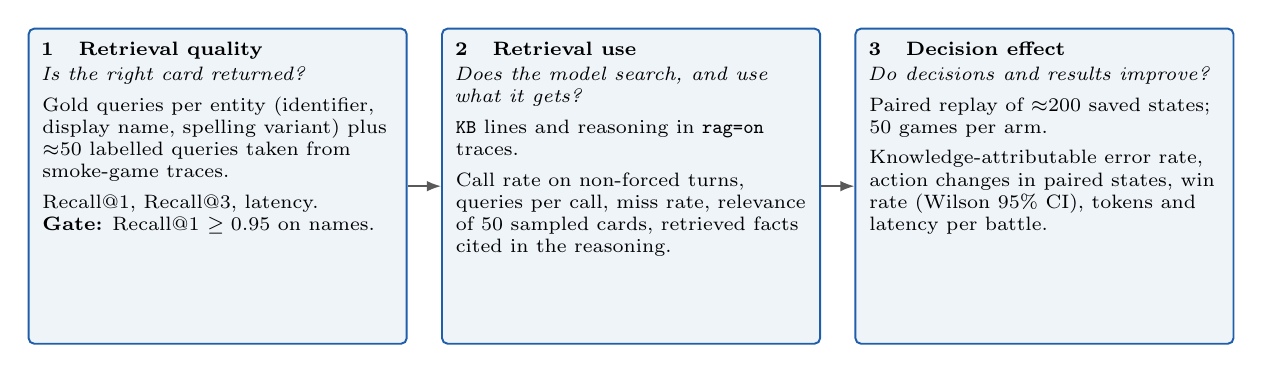
\begin{tikzpicture}[x=1cm, y=1cm,
  stage/.style={draw=ragblue, rounded corners=2pt, fill=ragfill, line width=0.7pt,
                inner sep=5pt, font=\scriptsize}]
  \node[stage] (s1) at (0,0) {\parbox[t][3.65cm][t]{4.45cm}{\raggedright \textbf{1\quad Retrieval quality}\\[1pt]
     \emph{Is the right card returned?}\\[3pt]
     Gold queries per entity (identifier, display name, spelling variant) plus ${\approx}50$ labelled
     queries taken from smoke-game traces.\\[3pt]
     Recall@1, Recall@3, latency.\\
     \textbf{Gate:} Recall@1 $\geq 0.95$ on names.}};
  \node[stage] (s2) at (5.25,0) {\parbox[t][3.65cm][t]{4.45cm}{\raggedright \textbf{2\quad Retrieval use}\\[1pt]
     \emph{Does the model search, and use what it gets?}\\[3pt]
     \code{KB} lines and reasoning in \code{rag=on} traces.\\[3pt]
     Call rate on non-forced turns, queries per call, miss rate, relevance of 50 sampled cards,
     retrieved facts cited in the reasoning.}};
  \node[stage] (s3) at (10.5,0) {\parbox[t][3.65cm][t]{4.45cm}{\raggedright \textbf{3\quad Decision effect}\\[1pt]
     \emph{Do decisions and results improve?}\\[3pt]
     Paired replay of ${\approx}200$ saved states; 50 games per arm.\\[3pt]
     Knowledge-attributable error rate, action changes in paired states, win rate (Wilson 95\% CI),
     tokens and latency per battle.}};
  \draw[arr] (s1) -- (s2);
  \draw[arr] (s2) -- (s3);
\end{tikzpicture}
\caption{Evaluation follows the retrieval chain. Each level explains the next: a weak decision effect is
attributed to retrieval quality, to retrieval use, or to the knowledge itself.}
\label{fig:eval}
\end{figure}

\begin{enumerate}
  \item \textbf{Retrieval quality} is checked offline, without calling the LLM, and acts as a gate: games
        start only when name queries reach Recall@1 of 0.95. If they do not, the cards or query construction
        are revised; the retrieval path is not changed.
  \item \textbf{Retrieval use} is read from the \code{rag=on} traces. A low call rate is itself a finding
        about how the model uses retrieval.
  \item \textbf{Decision effect} rests on two measures that are more sensitive than the win rate. The
        \emph{knowledge-attributable error rate} counts mistakes that knowledge would have prevented and that
        are visible in the battle log, for example a move absorbed by an ability (an \code{-immune} event
        attributed to Levitate, Flash Fire or Water Absorb). In \emph{paired replay}, battle states saved
        during \code{rag=off} games are decided again with retrieval enabled, so both arms are compared on
        identical positions.
\end{enumerate}

Win rates are reported with Wilson 95\% intervals. With 50 games per arm the interval around a 50\% win rate
is about $\pm 13$ percentage points, and a difference must reach about 27 points to be detected with 80\%
power. The win rate therefore confirms the direction of an effect; the claim rests on levels~2 and~3. Token
usage and latency are averaged per battle and reported as the cost of retrieval.

\subsection{Performance tuning outside the comparison}
\label{sec:tuning}
The thinking level (on or off, and its effort) and the wording of the reasoning instructions are tuned on a
few games to reduce latency and tokens. Two prompt defects are corrected at the same time: the opponent rating
is hard-coded to 1200, and the effective-power estimate scales the opponent's defence by our own stat boosts.
All of these settings are frozen before the comparison starts and are identical in both arms, so they
cannot account for a difference between them.

\section{Schedule and risks}
\label{sec:schedule}

Development ends on 15 November, in line with the plan agreed on 19 October, and games start only after the
retrieval gate is passed (Figure~\ref{fig:gantt}).

\begin{figure}[t]
\centering
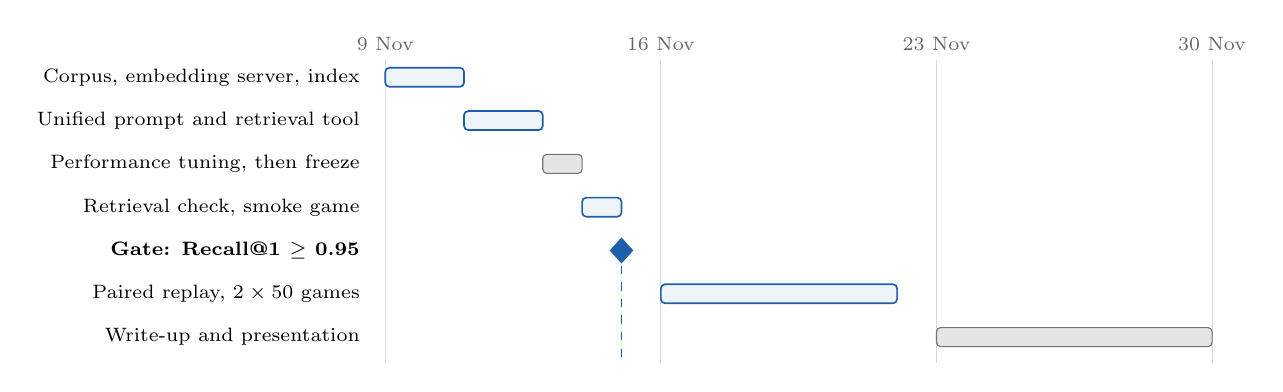
\begin{tikzpicture}[x=0.5cm, y=0.55cm, font=\scriptsize]
  % x = day - 9 (9 November = 0); y = -row
  \foreach \d/\t in {0/9 Nov, 7/16 Nov, 14/23 Nov, 21/30 Nov} {
    \draw[black!15] (\d,0.4) -- (\d,-6.6);
    \node[black!60, above] at (\d,0.4) {\t};
  }
  \newcommand{\task}[4]{% row, start, end, label
    \node[anchor=east] at (-0.4,-#1) {#4};
    \fill[black!10, rounded corners=1.5pt] (#2,-#1-0.22) rectangle (#3,-#1+0.22);
    \draw[edge, rounded corners=1.5pt] (#2,-#1-0.22) rectangle (#3,-#1+0.22);}
  \newcommand{\ragtask}[4]{%
    \node[anchor=east] at (-0.4,-#1) {#4};
    \fill[ragfill, rounded corners=1.5pt] (#2,-#1-0.22) rectangle (#3,-#1+0.22);
    \draw[ragblue, rounded corners=1.5pt, line width=0.6pt] (#2,-#1-0.22) rectangle (#3,-#1+0.22);}
  \ragtask{0}{0}{2}{Corpus, embedding server, index}
  \ragtask{1}{2}{4}{Unified prompt and retrieval tool}
  \task{2}{4}{5}{Performance tuning, then freeze}
  \ragtask{3}{5}{6}{Retrieval check, smoke game}
  \node[anchor=east] at (-0.4,-4) {\textbf{Gate: Recall@1 $\geq$ 0.95}};
  \fill[ragblue] (6,-4.3) -- (6.3,-4) -- (6,-3.7) -- (5.7,-4) -- cycle;
  \draw[ragblue, dashed] (6,-4.35) -- (6,-6.6);
  \ragtask{5}{7}{13}{Paired replay, $2\times50$ games}
  \task{6}{14}{21}{Write-up and presentation}
\end{tikzpicture}
\caption{Schedule for November 2026. Blue bars belong to the retrieval work; grey bars are tuning and
reporting. Games start only after the retrieval gate on 15 November.}
\label{fig:gantt}
\end{figure}

\begin{itemize}
  \item \textbf{The model rarely retrieves.} The \code{rag=on} arm would then behave like \code{rag=off}.
        The call rate is measured in the smoke game, and only the tool description is adjusted, before the
        settings are frozen.
  \item \textbf{Retrieval adds latency.} An extra tool round trip lengthens turns that already reach 73\,s.
        Batched queries and the card length limit bound the cost, and retrieval time is logged separately.
  \item \textbf{The embedding server fails during a run.} The tool then reports that knowledge is
        unavailable and the game continues. Such games are counted as invalid, and the index is checked with
        \code{knowledge\_doctor} before each batch.
  \item \textbf{Untested interfaces.} The parameters of \code{pi-knowledge}'s indexing and path-filter
        options are now exercised in this checkout by \code{pi\_agent.index\_kb}; the remaining gaps are
        cross-checking Recall@1, smoke-game latency and paired replay.
\end{itemize}

\section{Conclusion}

We have a working \code{pi\_agent} runtime: OpenCode Go as the default model, one deterministic knowledge
corpus, and a retrieval-enabled A/B comparison path that only toggles \code{search\_knowledge}. The next milestones are a
retrieval check that passes the Recall@1 gate, the paired replay set, and the first paired comparison
with confidence intervals.

\begin{thebibliography}{10}
\small
\raggedright
\setlength{\itemsep}{0pt}
\bibitem{pokechamp} S.~Karten et al., ``Pok\'eChamp: an Expert-level Minimax Language Agent,'' ICML 2025.
  \url{https://github.com/sethkarten/pokechamp}
\bibitem{rag} P.~Lewis et al., ``Retrieval-Augmented Generation for Knowledge-Intensive NLP Tasks,''
  NeurIPS 2020.
\bibitem{qwen3emb} Y.~Zhang et al., ``Qwen3 Embedding: Advancing Text Embedding and Reranking Through
  Foundation Models,'' arXiv:2506.05176, 2025.
\bibitem{tei} Hugging Face, Text Embeddings Inference. \url{https://github.com/huggingface/text-embeddings-inference}
\bibitem{vllm} W.~Kwon et al., ``Efficient Memory Management for Large Language Model Serving with
  PagedAttention,'' SOSP 2023.
\bibitem{pokeenv} \code{poke-env}: a Pok\'emon Showdown API for Python.
  \url{https://github.com/hsahovic/poke-env}
\bibitem{pi} \code{pi-python-core}: agent runtime used by \code{pi\_agent}.
  \url{https://pypi.org/project/pi-python-core/}
\bibitem{piknowledge} \code{pi-knowledge}: local knowledge base extension for Pi agents.
  \url{https://www.npmjs.com/package/pi-knowledge}
\bibitem{opencode} OpenCode Console Chat Completions API adapter.
  \url{https://opencode.ai/docs/api}

\bibitem{deepseek} DeepSeek API documentation (\code{deepseek-flash}, Responses API).
  \url{https://api-docs.deepseek.com}
\bibitem{challenge} PokeAgent Challenge: LLM Pok\'emon battle benchmark (public server closed).
  \url{https://pokeagentchallenge.com}
\end{thebibliography}

\end{document}
